\documentclass{article}
\usepackage[UTF8]{ctex}

\usepackage{amsmath}        %数学公式
\usepackage{amssymb}
\usepackage{cases}          %联立编号
\usepackage{cite}           %引用

\usepackage{graphicx}       %插入图片
\usepackage{float}          %设置图片浮动位置
\usepackage{subfigure}      %插入多图时用子图显示

\usepackage{listings}
\usepackage{xcolor}

\usepackage{anyfontsize}    %解决一个奇怪的字体大小报错问题
\usepackage{fancyhdr}       %页眉、页脚、页码
\usepackage[a4paper, margin=1in]{geometry}    %纸张大小
\usepackage{longtable}

\lstset{
    basicstyle          =   \sffamily,          % 基本代码风格
    keywordstyle        =   \bfseries,          % 关键字风格
    commentstyle        =   \rmfamily\itshape,  % 注释的风格,斜体
    stringstyle         =   \ttfamily,  % 字符串风格
    flexiblecolumns,                % 别问为什么,加上这个
    numbers             =   left,   % 行号的位置在左边
    showspaces          =   false,  % 是否显示空格,显示了有点乱,所以不现实了
    numberstyle         =   \zihao{-5}\ttfamily,    % 行号的样式,小五号,tt等宽字体
    showstringspaces    =   false,
    captionpos          =   t,      % 这段代码的名字所呈现的位置,t指的是top上面
    frame               =   lrtb,   % 显示边框
}

\lstdefinestyle{Python}{
    language        =   Python, % 语言选Python
    basicstyle      =   \zihao{-5}\ttfamily,
    numberstyle     =   \zihao{-5}\ttfamily,
    keywordstyle    =   \color{blue},
    keywordstyle    =   [2] \color{teal},
    stringstyle     =   \color{magenta},
    commentstyle    =   \color{red}\ttfamily,
    breaklines      =   true,   % 自动换行,建议不要写太长的行
    columns         =   fixed,  % 如果不加这一句,字间距就不固定,很丑,必须加
    basewidth       =   0.5em,
}

\newcommand\f[2]{\frac{#1}{#2}}
\newcommand\pf[2]{\frac{\partial#1}{\partial#2}}
\newcommand\df[2]{\dfrac{#1}{#2}}
\newcommand\pdf[2]{\dfrac{\partial#1}{\partial#2}}

\title{\bf\huge 概率论与数理统计 - 作业 3}
\author{Jerry}
\date{\today}

\begin{document}
\maketitle

\section*{T1. }

\subsubsection*{(1. )}

例子:随机扔一个骰子,得到的数字

随机变量的类型:离散型随机变量

样本空间:\{1,2,3,4,5,6\}

\subsubsection*{(2. )}

例子:1天内某路口交通事故数量

随机变量的类型:离散型随机变量

样本空间:\{0,1,2,...,n\}

\subsubsection*{(3. )}

例子:某个设备正常工作的时间

随机变量的类型:连续型随机变量

样本空间:[0,+$\infty$)

\subsubsection*{(4. )}

例子:半径为$a$的圆弧上随机取两点连成的弧长

随机变量的类型:连续型随机变量

样本空间:[0,2$a$]

\subsubsection*{(5. )}

例子:1$s$内某个水龙头流出的水量

随机变量的类型:连续型随机变量

样本空间:[0,+$\infty$)

\section*{T2. }

$F(x)=P(X\leq x)$

\subsubsection*{(1. )}

$F(x)$为单调递增函数

假设$lim_{x\to-\infty}F(x)>0$,则我们可以认为$F(x)$在$x\to-\infty$收敛于$a>0$,可以推出概率和小于1,与概率之和为$1$不符

假设$lim_{x\to\infty}F(x)<1$,则我们可以认为$F(x)$在$x\to\infty$收敛于$b<1$,可以推出概率和小于1,与概率之和为$1$不符

\subsubsection*{(2. )}

我们构建一个数列$\{x_n\}=x_0+\f{1}{n}$,证明$\lim_{n\to\infty}F(x_n)=F(x)$即可

\begin{equation}
    \begin{aligned}
        F(x_1)-F(x_0)
        & =P(x_0<X\leq x_1)\\
        & =P(\bigcup_{i=1}^\infty x_{i+1}<X\leq x_i)\\
        & =\sum_{i=1}^{\infty}P(x_{i+1}<X\leq x_i)\\
        & =\sum_{i=1}^{\infty}[F(x_i)-F(x_{i+1})]\\
        & =\lim_{i\to\infty}[F(x_1)-F(x_{i+1})]\\
        & =F(x_1)-\lim_{i\to\infty}F(x_i)
    \end{aligned}
\end{equation}

故有$F(x_0)=\lim_{i\to\infty}F(x_i)$,即函数右连续

\subsubsection*{(3. )}

$F(b)-F(a)=P(a< X\leq b)$

故$P(a\leq X\leq b)=F(b)-F(a)+P(X=a)=F(b)-F(a)+[F(a)-F(a^-)]=F(b)-F(a^-)$

% 由于函数右连续,故$P(X\leq a)=P(X<a)$

\section*{T3. }

\subsubsection*{(1. )}

$\Omega=\omega_1,\omega_2,\omega_3;X=1,2,3;Y=1,2,3$

$P(X=1)=P(\omega_1)=\f{1}{3},P(X=2)=P(\omega_2)=\f{1}{3},P(X=3)=P(\omega_3)=\f{1}{3}$

$P(Y=1)=P(\omega_3)=\f{1}{3},P(Y=2)=P(\omega_1)=\f{1}{3},P(Y=3)=P(\omega_2)=\f{1}{3}$

故$X,Y$两个随机变量分布相同

\subsubsection*{(2. )}

$\Omega=\omega_1,\omega_2,\omega_3;X+Y=3,5,4;X-Y=-1,-1,2$

$P(X+Y=3)=P(\omega_1)=\f{1}{3},P(X+Y=5)=P(\omega_2)=\f{1}{3},P(X+Y=4)=P(\omega_3)=\f{1}{3}$

$P(X-Y=-1)=P(\omega_1+\omega_2)=\f{2}{3},P(X-Y=2)=P(\omega_3)=\f{1}{3}$

\begin{table}[H]
    \centering
    \begin{tabular}{|l|l|l|l|}
        \hline
        $X+Y$ & ~~$3$~~ & ~~$4$~~ & ~~$5$~~ \\ \hline
        $P(X+Y)$ & ~~$\f{1}{3}$ & ~~$\f{1}{3}$ & ~~$\f{1}{3}$ \\ \hline
    \end{tabular}
\end{table}

\begin{table}[H]
    \centering
    \begin{tabular}{|l|l|l|}
        \hline
        $X-Y$ & ~~$-1$~~ & ~~$2$~~ \\ \hline
        $P(X-Y)$ & ~~$\f{2}{3}$ & ~~$\f{1}{3}$ \\ \hline
    \end{tabular}
\end{table}

\section*{T4. }

证明:

$E(X^2)=\sum_{i=1}^{N}x_i^2p_i$

$E(X)=\sum_{i=1}^{N}x_ip_i$

\begin{equation}
    \begin{aligned}
        Var(X)
        & =\sum_{i=1}^{N}(x_i-E(x))^2p_i\\
        & =\sum_{i=1}^{N}x_i^2p_i-\sum_{i=1}^{N}2x_ip_iE(X)+\sum_{i=1}^{N}E(X)^2p_i\\
        & =E(X^2)-2E(X)\sum_{i=1}^{N}x_ip_i+E(X)^2\\
        & =E(X^2)-2E(X)E(X)+E(X)^2\\
        & =E(X^2)-2E(X)^2+E(X)^2\\
        & =E(X^2)-E(X)^2
    \end{aligned}
\end{equation}

不一致,但是均在刻画数据的集中程度

\section*{T5. }

\subsubsection*{(1. )}

$$P(X=n)=P(N_n)P(Y_{n+1})=\df{C^n_a}{C^n_{a+b}}\df{1}{b}$$

\subsubsection*{(2. )}

$$P(X=n)=P(N_n)P(Y_{n+1})=(\df{C^1_a}{C^1_{a+b}})^n\df{1}{b}=(\df{a}{a+b})^n\df{1}{b}$$

\begin{equation}
    \begin{aligned}
        E(X)
        & =\lim_{N\to \infty}\sum_{i=1}^{N}i(\df{a}{a+b})^i\df{1}{b}\\
        & =\df{1}{b}\lim_{N\to\infty}\sum_{i=1}^{N}i\cdot(\df{a}{a+b})^i\\
        & =\df{1}{b}\lim_{N\to\infty}\df{\df{\f{a}{a+b}-(\f{a}{a+b})^{N+1}}{1-\f{a}{a+b}}-n(\f{a}{a+b})^{N+1}}{1-\f{a}{a+b}}\\
        & =\df{1}{b}\cdot\df{\f{\f{a}{a+b}-0}{\f{b}{a+b}}-0}{\f{b}{a+b}}\\
        % & =\df{1}{b}\cdot\df{\f{a}{a+b}\cdot\f{a+b}{b}}{\f{b}{a+b}}\\
        & =\df{a}{b}(a+b)
    \end{aligned}
\end{equation}

\section*{T6. }

存在。理由如下:

构造$X=\{1,1000\}$,$P(X=1)=0.99$,$P(X=1000)=0.01$,$Y=2$

有$E(X)>10>2=E(B)$,$P(Y>X)=P(X<2)=0.99$

\section*{T7. }

\subsubsection*{(1. )}

$$P(X=n)=P(N_{n-1})P(Y_n)=(1-p)^{n-1}p$$

\subsubsection*{(2. )}

$\sum_{n=0}^{\infty}n(1-p)^n=\lim_{n\to \infty}\df{\df{(1-p)-(1-p)^{n+1}}{1-(1-p)}-n(1-p)^{n+1}}{1-(1-p)}=\df{\df{1-p}{p}}{p}=\df{1-p}{p^2}$

\begin{equation}
    \begin{aligned}
        E(X)
        & =\sum_{n=0}^{\infty}nP(X=n)\\
        & =\sum_{n=0}^{\infty}np(1-p)^{n-1}\\
        & =\f{p}{1-p}\sum_{n=0}^{\infty}n(1-p)^n\\
        & =\df{p}{1-p}\df{1-p}{p^2}\\
        & =\df{1}{p}
    \end{aligned}
\end{equation}

$\sum_{n=0}^{\infty}n^2(1-p)^n=\lim_{n \to \infty}\df{(1-p)(-(n^2(2-p)^2-2n(2-p)+2-p)(1-p)^n+2-p)}{p^3}=\df{(1-p)(2-p)}{p^3}$

\begin{equation}
    \begin{aligned}
        E(X^2)
        & =\sum_{n=0}^{\infty}n^2P(X=n)\\
        & =\sum_{n=0}^{\infty}n^2p(1-p)^{n-1}\\
        & =\df{p}{1-p}\sum_{n=0}^{\infty}n^2(1-p)^n\\
        & =\df{p}{1-p}\df{(1-p)(2-p)}{p^3}\\
        & =\df{2-p}{p^2}
    \end{aligned}
\end{equation}

$Var(X)=E(X^2)-(E(x))^2=\df{2-p}{p^2}-\df{1}{p^2}=\df{1-p}{p^2}$

\section*{T8. }

\subsubsection*{(1. )}

$P(X\geq15)=\sum_{i=15}^{25}P(X=i)=\sum_{i=15}^{25}C_{25}^i(\df{3}{5})^i(\df{2}{5})^{25-i}$,

\subsubsection*{(2. )}

$P(X>20)=\sum_{i=21}^{25}P(X=i)=\sum_{i=21}^{25}C_{25}^i(\df{3}{5})^i(\df{2}{5})^{25-i}$,

\subsubsection*{(3. )}

$P(X<10)=\sum_{i=1}^{9}P(X=i)=\sum_{i=1}^{9}C_{25}^i(\df{3}{5})^i(\df{2}{5})^{25-i}$,

\section*{T9. }

计算二项分布$B(n,p)$的期望与方差

\begin{equation}
    \begin{aligned}
        E(X)
        & = \sum_{k=0}^{n}kp_k\\
        % & = \sum_{k=0}^{n}kC_n^kp^k(1-p)^{n-k}\\
        & = \sum_{k=1}^{n}kC_n^kp^k(1-p)^{n-k}\\
        & = \sum_{k=1}^{n}k\df{n!}{k!(n-k)!}p^k(1-p)^{n-k}\\
        % & = np\sum_{k=1}^{n}\df{(n-1)!}{(k-1)!(n-k)!}p^{k-1}(1-p)^{n-k}\\
        & = np\sum_{(k-1)=0}^{(n-1)}\df{(n-1)!}{(k-1)!((n-1)-(k-1))!}p^{(k-1)}(1-p)^{(n-1)-(k-1)}\\
        & = np\sum_{(k-1)=0}^{(n-1)}C_{(n-1)}^{(k-1)}p^{(k-1)}(1-p)^{(n-1)-(k-1)}\\
        & = np
    \end{aligned}
\end{equation}

\begin{equation}
    \begin{aligned}
        E(X^2)
        & = \sum_{k=0}^{n}k^2p_k\\
        % & = \sum_{k=0}^{n}k(k-1+1)C_n^kp^k(1-p)^{n-k}\\
        & = \sum_{k=1}^{n}k(k-1)C_n^kp^k(1-p)^{n-k}+\sum_{k=1}^{n}kC_n^kp^k(1-p)^{n-k}\\
        & = \sum_{k=1}^{n}k(k-1)\df{n!}{k!(n-k)!}p^k(1-p)^{n-k}+E(X)\\
        & = n(n-1)p^2\sum_{k=2}^{n}\df{(n-2)!}{(k-2)!(n-k)!}p^{k-2}(1-p)^{n-k}+E(X)\\
        & = n(n-1)p^2\sum_{(k-2)=0}^{(n-2)}\df{(n-2)!}{(k-2)!(n-k)!}p^{(k-2)}(1-p)^{(n-2)-(k-2)}+E(X)\\
        & = n(n-1)p^2\sum_{(k-2)=0}^{(n-2)}C_{n-2}^{k-2}p^{(k-2)}(1-p)^{(n-2)-(k-2)}+E(X)\\
        & = n(n-1)p^2+np
    \end{aligned}
\end{equation}

故

\begin{equation}
    \begin{aligned}
        Var(X)
        & = E(X^2)-E(X)^2\\
        & = n(n-1)p^2+np-(np)^2\\
        & = n^2p^2-np^2+np-n^2p^2\\
        & = np(1-p)
    \end{aligned}
\end{equation}

\section*{T10. }

\subsubsection*{(1. )}

$P(X=m)=\df{C_M^m C_{N-M}^{n-m}}{C_N^n}$

\subsubsection*{(2. )}

在充分混合后,我们可以认为这个样本中标记的鱼的比例与整个池子中标记的鱼的比例相同,
故$\f{M}{N}=\f{m}{n}$,计算得$N=\f{n}{m}\cdot M$

\subsubsection*{(3. )}

$P(X=m)=\df{C_M^m C_{N-M}^{n-m}}{C_N^n}=\df{\f{M!}{m!(M-m)!}\cdot\f{(N-M)!}{(n-m)!(N-M-n+m)!}}{\f{N!}{n!(N-n)!}}=F(m,n,M)\cdot G(N)$

其中,$G(N)=\df{(N-n)!(N-M)!}{N!(N-M-n+m)!}$

$\df{G(N+1)}{G(N)}=\df{(N-n+1)!}{(N-n)!}\cdot\df{(N-M+1)!}{(N-M)!}\cdot\df{N!}{(N+1)!}\cdot\df{(N-M-n+m)!}{(N-M-n+m+1)!}=\df{(N-n+1)(N-M+1)}{(N+1)(N-M-n+m+1)}$

$\df{G(N+1)}{G(N)}$等于1的点即为最大值点,则$\df{(N-n+1)(N-M+1)}{(N+1)(N-M-n+m+1)}=1$,化简得$N=\f{n}{m}\cdot M$

\section*{T11. }

绘制图像如下:

\begin{center}
    \begin{figure}[H] %H为当前位置,!htb为忽略美学标准,htbp为浮动图形
        \centering %图片居中
        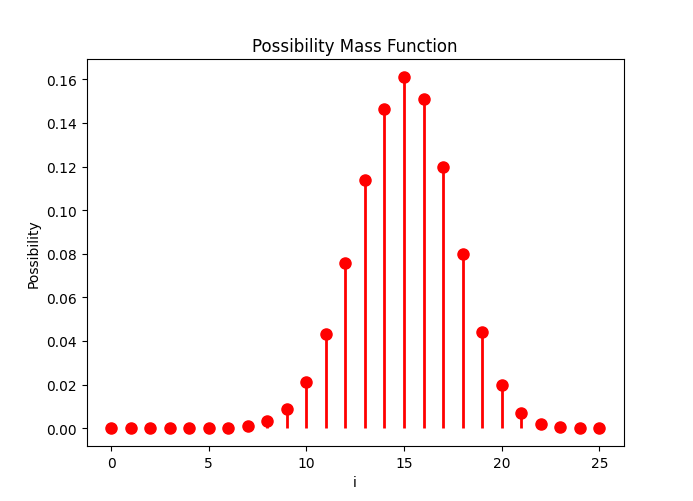
\includegraphics[width=0.5\textwidth]{img/Figure_1.png} %插入图片,[]中设置图片大小,{}中是图片文件名
        \caption{pmf} %最终文档中希望显示的图片标题
        \label{fig1} %用于文内引用的标签
    \end{figure}
\end{center}

\subsubsection*{(1. )}

在$x=15$时有最大概率$0.16115793869486378$

\subsubsection*{(2. )}

期望值$\mu=14.999999999999998$,在计算的误差允许范围内可以认为期望值与最大概率相等

\subsubsection*{(3. )}

方差$\sigma^2=6.000000000000002$

\subsubsection*{(4. )}

$\mu-2\sigma<x<\mu+2\sigma$的概率是0.9362462771170672

\subsubsection*{Code}

源代码如下:

\lstinputlisting[
    style       =   Python,
    caption     =   {\bf simulation1.py},
    label       =   {1}
]{code/simulation1.py}

除图像外运行结果如下:

The maximum possibility is 0.16115793869486378 when i = 15

The mathematical expectation is 14.999999999999998

The variance is 6.000000000000002

The possibility of $\mu-2\sigma<x<\mu+2\sigma$ is 0.9362462771170672

\end{document}
